\section{连续性}
\label{sec:ru-continuity}
\label{sec:analysis-local-models}
\label{sec:analysis-metric-continuity-extrema}

对$f(x)=x^2$，输入$x$接近$a$时，输出接近$a^2$，而$a^2$恰好是函数在$a$处的值。连续性描述的就是这种关系：输出趋近的目标等于函数在该点的取值。
本节先给出定义和运算性质，再研究闭区间上的连续函数为什么一定达到最值、取遍中间值，最后比较几种强弱不同的连续性条件。

\subsection{连续性的定义和性质}
\label{sec:ru-continuity-definition}

\begin{definition}[连续]
\label{def:analysis-continuity}
设$X\subseteq\mathbb R$，$f:X\to\mathbb R$，$a\in X$。若对每个$\varepsilon>0$，都存在$\delta>0$，使
\[
 x\in X,\quad|x-a|<\delta\quad\Longrightarrow\quad|f(x)-f(a)|<\varepsilon,
\]
则称$f$在$a$处\term{连续}（continuous）。若$f$在$X$的每一点连续，就称$f$为连续函数。
\end{definition}
与函数极限的定义相比，这里不排除$x=a$，因为目标值就是$f(a)$。连续性与极限的关系取决于$a$在定义域中的位置。
若$a$是$X$的聚点，连续等价于$\lim_{x\to a}f(x)=f(a)$；若$a$是孤立点，取$\delta$足够小，使邻域内属于$X$的点只有$a$，条件自动成立；
若$a$是闭区间的端点，连续就是相应的单侧极限等于函数值。

用定义验证连续性时，需要对每个$\varepsilon$具体找出$\delta$。
\begin{example}[平方函数在每一点连续]
\label{ex:analysis-square-pointwise-continuity}
设$f(x)=x^2$，固定$a$。若$|x-a|<1$，则$|x+a|\leq|x-a|+2|a|<2|a|+1$，从而$|x^2-a^2|=|x-a|\,|x+a|\leq(2|a|+1)|x-a|$。
给定$\varepsilon>0$，取$\delta=\min\{1,\varepsilon/(2|a|+1)\}$，则$|x-a|<\delta$时$|x^2-a^2|<\varepsilon$。
\end{example}
例中的$\delta$随$|a|$增大而缩小：基点离原点越远，图像越陡，允许的输入误差越小。第~\ref{sec:analysis-continuity-relations}节将说明，在整条实轴上这种依赖无法消除。

不连续的点称为间断点，按失效方式可以分为几类。若$\lim_{x\to a}f(x)$存在但不等于$f(a)$，称为可去间断：改变$f(a)$的值，函数便连续，例如把$x^2$在$0$处的值改为$1$。
若左右极限都存在但不相等，称为跳跃间断，例如阶跃函数$\mathbb I\{x\geq0\}$在$0$处。两类并未穷尽所有情形：令$f(0)=0$、$x\neq0$时$f(x)=\sin(1/x)$，上一节已看到它在$0$处连单侧极限都不存在，这是振荡导致的间断。

连续性可以用序列刻画：$f$在$a\in X$处连续，当且仅当对每列满足$x_n\in X$、$x_n\to a$的输入，都有$f(x_n)\to f(a)$。证明与函数极限的序列判据相同，只是不必排除$x_n=a$。
由此，函数极限的运算法则直接给出：$f,g$在$a$处连续时，$f\pm g$、$fg$、$cf$在$a$处连续；若还有$g(a)\neq0$，则$f/g$在$a$附近有定义并在$a$处连续。
复合同样保持连续：若$f$在$a$处连续，$g$在$f(a)$处连续，则$g\circ f$在$a$处连续。给定$\varepsilon$，先由$g$的连续性得到$\eta$，再由$f$的连续性取$\delta$使$|f(x)-f(a)|<\eta$，两步误差传递便连成一步。
与复合函数的极限不同，这里外层在$f(a)$处连续，所以不需要额外条件。由这些规则，多项式在$\mathbb R$上连续，有理函数在分母非零处连续。
本节只用实轴上的绝对值距离；把输入和输出的距离换成一般的度量，就得到第~\ref{chap:metric-spaces}章中一般映射的连续性。

\subsection{闭区间上连续函数的性质}
\label{sec:ru-closed-interval-continuity}
\label{sec:analysis-metric-measurement}
\label{sec:analysis-set-metric}

函数$f(x)=x$在$(0,1)$上连续，却没有最小值；在$[0,1]$上则有。区别来自定义域：$(0,1)$中的点列$1/n$趋于$0$，极限却不在定义域内。
要从各点的局部性质得到整个定义域上的结论，需要先描述哪些集合能留住其中点列的极限，以及怎样把局部控制合成整体控制。

集合$U\subseteq\mathbb R$若对每个$x\in U$都存在$r>0$使$(x-r,x+r)\subseteq U$，就称为\term{开集}（open set）；补集为开集的集合称为\term{闭集}（closed set）。
开区间是开集，闭区间是闭集；$[0,1)$既不开也不闭，$\mathbb R$与空集既开又闭。闭集的意义可以换成点列的语言来理解。
\begin{lemma}[闭集的序列判据]
\label{lem:analysis-closed-sequence-criterion}
$F\subseteq\mathbb R$是闭集，当且仅当：每个取值于$F$的收敛数列，其极限也属于$F$。
\end{lemma}
\begin{proof}
设$F$闭。若取值于$F$的数列收敛到$x\notin F$，开集$\mathbb R\setminus F$包含某个$(x-r,x+r)$，充分靠后的项都落在其中，与$x_n\in F$矛盾。
反之，若$F$不闭，补集不是开集，存在$x\notin F$使每个$(x-1/n,x+1/n)$都与$F$相交；从中各选一点$x_n\in F$，则$x_n\to x\notin F$。
\end{proof}
闭与有界是不同的性质：$(0,1)$有界但不闭，$\mathbb R$闭但无界。二者同时成立时，Bolzano--Weierstrass定理给出收敛子列，本引理又保证子列的极限仍在集合内。
这一“闭有界集中的点列有收敛到集合内的子列”的性质，是本小节各定理的共同依据。

同一性质还有另一种表达：把局部控制合成整体控制。若一族开集的并包含$K$，称它们为$K$的\term{开覆盖}（open cover）；若能从中选出有限个仍覆盖$K$，称为\term{有限子覆盖}（finite subcover）。
若$K$的每个开覆盖都有有限子覆盖，称$K$\term{紧致}（compact）。
\begin{theorem}[闭区间的有限子覆盖性质]
\label{thm:analysis-interval-finite-subcover}
实轴上的每个闭区间$[a,b]$都是紧致集。
\end{theorem}
\begin{proof}
设$a<b$，给定$[a,b]$的开覆盖$\mathcal U$。先证明存在一个共同尺度：
\begin{equation}
 \exists r>0,\quad\forall x\in[a,b],\quad\exists U\in\mathcal U,\qquad(x-r,x+r)\cap[a,b]\subseteq U.
 \label{eq:analysis-cover-uniform-radius}
\end{equation}
若不然，对每个$n$可选$x_n\in[a,b]$，使$(x_n-1/n,x_n+1/n)\cap[a,b]$不包含于任何覆盖成员。取收敛子列$x_{n_k}\to x\in[a,b]$，选$U\in\mathcal U$与$\rho>0$使$(x-\rho,x+\rho)\subseteq U$。
当$k$足够大时$|x_{n_k}-x|<\rho/2$且$1/n_k<\rho/2$，于是$(x_{n_k}-1/n_k,x_{n_k}+1/n_k)\subseteq U$，与选取矛盾。
有了共同半径$r$，把$[a,b]$分成有限个长度小于$r$的小段，每段落在某个$(x-r,x+r)$内，因而被一个覆盖成员包含；每段选一个成员即得有限子覆盖。
\end{proof}
图~\ref{fig:analysis-process-finite-open-cover}对照闭区间的有限覆盖与开区间上无法有限选取的覆盖。每个有界闭集也是紧致的：把它放进某个$[a,b]$，把它的补集加入开覆盖，应用定理后再删去补集即可。
有限子覆盖与收敛子列是同一性质的两种说法，后者在下面的证明中更直接，前者在需要把无限多个局部估计合成一个时更方便。

\begin{figure}[!htbp]
 \centering
 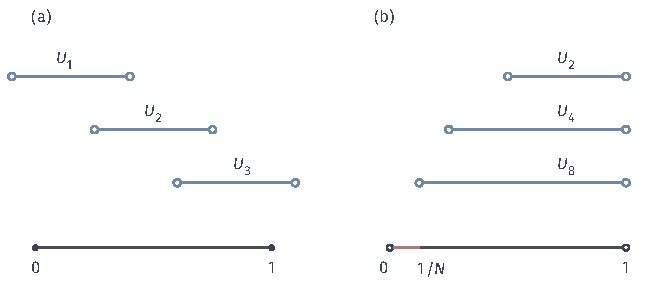
\includegraphics[width=112mm]{figures/01-mathematical-preliminaries-upper/00-shared/tikz/chapter3-concept-processes/finite-open-cover.pdf}
 \caption{(a) 三个开区间$(-0.1,0.4)$、$(0.25,0.75)$、$(0.6,1.1)$覆盖$[0,1]$。(b) $U_n=(1/n,1)$（$n\geq2$）覆盖$(0,1)$；只选有限多个时，设最大下标为$N$，红段$(0,1/N]$仍未覆盖。图只画$U_2,U_4,U_8$；右侧的失败由最大下标论证，不是有限图像的猜测。}
 \label{fig:analysis-process-finite-open-cover}
\end{figure}

\begin{theorem}[极值定理]
\label{thm:analysis-extreme-value}
设$K\subseteq\mathbb R$非空、闭且有界，$f:K\to\mathbb R$连续，则$f$有界，并在$K$上达到最小值和最大值。
\end{theorem}
\begin{proof}
若$f$无界，可选$x_n\in K$使$|f(x_n)|>n$；取收敛子列$x_{n_k}\to x\in K$，连续性给出$f(x_{n_k})\to f(x)$，收敛数列有界，与$|f(x_{n_k})|>n_k$矛盾。
于是$m=\inf_Kf$是有限实数。对每个$n$选$x_n\in K$使$m\leq f(x_n)<m+1/n$，取收敛子列$x_{n_k}\to x^\star\in K$，则$f(x_{n_k})\to f(x^\star)$，同时$f(x_{n_k})\to m$，所以$f(x^\star)=m$。对$-f$重复论证即得最大值。
\end{proof}
三个条件各排除一种失效方式：有界保证收敛子列，闭保证子列的极限仍在定义域内，连续保证函数值随之收敛。下面三个例子各缺一个条件，下确界都取不到。
\begin{example}[极值定理的条件]
\label{ex:analysis-extrema-failures}
定义域不闭：$f(x)=x$在$(0,1)$上的下确界$0$不被取得。定义域无界：$e^x$在$\mathbb R$上连续，下确界为$0$，但$e^x>0$，取不到。
函数不连续：在$[0,1]$上令$f(0)=1$、$x>0$时$f(x)=x$，下确界为$0$，而$f$在每一点的值都大于$0$。
\end{example}

另一条整体性质说的是：函数从一个值变到另一个值时，要经过中间的每个值。这要求两端之间的整段都属于定义域。
\begin{theorem}[介值定理]
\label{thm:analysis-intermediate-value}
设$a<b$，$f:[a,b]\to\mathbb R$连续。则对介于$f(a)$与$f(b)$之间的每个$c$，都存在$\xi\in[a,b]$使$f(\xi)=c$；若$c$严格位于二者之间，可取$\xi\in(a,b)$。
\end{theorem}
\begin{proof}
设$f(a)<c<f(b)$（端点值相等的情形直接取端点，$f(a)>f(b)$时考虑$-f$）。令$S=\{x\in[a,b]:f(x)\leq c\}$，它含$a$且以$b$为上界，由确界原理$u=\sup S$存在。
取$x_n\in S$使$x_n\to u$，连续性给出$f(u)\leq c$，因而$u\neq b$。若$f(u)<c$，由连续性，$u$右侧充分近的点仍满足$f<c$，它们属于$S$却大于$u$，矛盾。所以$f(u)=c$，又由$f(a)<c$知$u\neq a$。
\end{proof}
证明用到了区间不缺中间点：确界$u$仍在区间中，并且$u$的右侧还有区间内的点。定义域闭且有界但有缺口时，介值性可能失效。
\begin{example}[有缺口的定义域上不取中间值]
\label{ex:analysis-intermediate-value-gap}
令$X=[-2,-1]\cup[1,2]$，在$[-2,-1]$上取$f=0$，在$[1,2]$上取$f=1$。对每个$a\in X$取$\delta=1$，邻域内属于$X$的点与$a$在同一段，所以$f$连续。$X$闭且有界，$f$却不取$1/2$。
\end{example}
这个函数在$X$上仍然达到最值：闭有界足以保证最值，却不能代替介值定理的区间条件。

介值定理最直接的用途是证明方程有解。若$f$在$[a,b]$上连续且$f(a)f(b)<0$，则$f$在$(a,b)$内有零点。这个结论还给出求零点的方法，即\term{二分法}（bisection method）：
取中点$m=(a+b)/2$，若$f(m)=0$则停止，否则保留端点函数值异号的那一半，重复进行。$n$步后零点落在长度为$(b-a)/2^n$的区间内，取该区间中点作为近似值，误差不超过$(b-a)/2^{n+1}$。
例如$f(x)=x^2-2$在$[1,2]$上两端异号，第一步$f(1.5)=0.25>0$保留$[1,1.5]$，第二步$f(1.25)<0$保留$[1.25,1.5]$；要使误差小于$10^{-6}$，约需$20$步。
二分法只用到连续性和符号，不需要导数；所需步数由误差界事先确定。

介值定理还说明，区间上的连续函数把区间映成区间：若$f(I)$中有$y_1<y_2$，它们之间的每个值也被取到。由此可以研究反函数的连续性。
\begin{theorem}[严格单调连续函数的反函数]
\label{thm:ru-inverse-continuity}
\label{sec:analysis-inverse-continuity}
设$f$在区间$I$上连续且严格单调，则$f(I)$是区间，$f:I\to f(I)$是双射，并且反函数$f^{-1}$在$f(I)$上连续、与$f$同向严格单调。
\end{theorem}
\begin{proof}
双射与单调性已在第~\ref{sec:ru-function-properties}节说明，$f(I)$是区间由介值定理得到。以严格递增、$a$为$I$的内点为例，给定足够小的$\varepsilon>0$使$a\pm\varepsilon\in I$，有$f(a-\varepsilon)<f(a)<f(a+\varepsilon)$。
取$\delta=\min\{f(a)-f(a-\varepsilon),\,f(a+\varepsilon)-f(a)\}$，若$y\in f(I)$且$|y-f(a)|<\delta$，则$f(a-\varepsilon)<y<f(a+\varepsilon)$，严格递增迫使$f^{-1}(y)\in(a-\varepsilon,a+\varepsilon)$。端点只在一侧取点，论证相同。
\end{proof}

现在可以严格构造自然对数。上一节已经得到：$e^x$严格递增，$x\to-\infty$时趋于$0$，$x\to+\infty$时趋于$+\infty$，并且$|e^{x+h}-e^x|\leq e^x(|h|+2h^2)$，所以它在每一点连续。
对任意$y>0$，先取两个输入使指数值分别小于和大于$y$，再用介值定理得到原像；严格单调保证原像唯一。所以$e^x$是$\mathbb R$到$(0,+\infty)$的双射，它的反函数称为\term{自然对数}（natural logarithm），记作$\log x$，定义在$x>0$上。
由定理~\ref{thm:ru-inverse-continuity}，$\log$连续且严格递增；由指数的加法公式，$\log(xy)=\log x+\log y$。对$a>0$与实数$x$，定义$a^x=e^{x\log a}$，它对整数$x$与通常的乘幂一致。
这样，上一章作为背景使用的指数—对数关系，现在都有了依据。

\subsection{一致连续与Lipschitz连续}
\label{sec:ru-uniform-lipschitz}
\label{sec:analysis-continuity-relations}

连续性定义中的$\delta$可以随基点改变，平方函数的例子中$\delta$就随$|a|$增大而缩小。若要求同一个$\delta$适用于整个定义域，或者要求输出误差不超过输入误差的固定倍数，就得到更强的条件。
\begin{definition}[一致连续]
\label{def:analysis-uniform-continuity}
函数$f:X\to\mathbb R$称为\term{一致连续}（uniformly continuous），若对每个$\varepsilon>0$，都存在$\delta>0$，使任意$x,y\in X$满足$|x-y|<\delta$时都有$|f(x)-f(y)|<\varepsilon$。
\end{definition}
与逐点连续相比，变化在于量词的次序：逐点连续是“对每个点和每个$\varepsilon$，存在$\delta$”，一致连续是“对每个$\varepsilon$，存在对所有点都有效的$\delta$”。
\begin{example}[平方函数在实轴上不一致连续]
\label{ex:analysis-square-not-uniformly-continuous}
取$x_n=n$、$y_n=n+1/n$，则$|y_n-x_n|=1/n\to0$，而$y_n^2-x_n^2=2+1/n^2>2$。若平方函数在$\mathbb R$上一致连续，对$\varepsilon=1$取$\delta$，当$n>1/\delta$时便与上式矛盾。
\end{example}
两列点都逃向无穷远，那里平方函数越来越陡。把定义域限制在$[0,1]$上，则$|x^2-y^2|=|x+y|\,|x-y|\leq2|x-y|$，取$\delta=\varepsilon/2$即可。
同一个函数在两个定义域上表现不同，原因在于逃向无穷远的点列在有界闭集中不存在。
\begin{theorem}[一致连续性定理]
\label{thm:analysis-uniform-continuity}
设$K\subseteq\mathbb R$非空、闭且有界，$f:K\to\mathbb R$连续，则$f$在$K$上一致连续。特别地，闭区间上的连续函数一致连续。
\end{theorem}
\begin{proof}
若不然，存在$\varepsilon_0>0$，使每个$\delta=1/n$都对应$x_n,y_n\in K$，满足$|x_n-y_n|<1/n$而$|f(x_n)-f(y_n)|\geq\varepsilon_0$。
取收敛子列$x_{n_k}\to x\in K$，则$y_{n_k}\to x$。由$f$在$x$处连续，$f(x_{n_k})$与$f(y_{n_k})$都趋于$f(x)$，两者之差趋于零，与$\varepsilon_0$矛盾。
\end{proof}

一致连续只断言共同的$\delta$存在，没有给出输出误差与输入误差的数量关系。若这个关系是线性的，误差控制就更具体。
\begin{definition}[Lipschitz连续]
\label{def:analysis-lipschitz-continuity}
若存在常数$L\geq0$，使所有$x,y\in X$都满足
\begin{equation}
 |f(x)-f(y)|\leq L|x-y|,
 \label{eq:analysis-lipschitz-condition}
\end{equation}
则称$f$为\term{Lipschitz连续}（Lipschitz continuous）函数，$L$称为一个Lipschitz常数。若每一点都有一个邻域，$f$在其中满足这一条件（常数可随邻域改变），称$f$\term{局部Lipschitz连续}（locally Lipschitz）。
\end{definition}
Lipschitz连续蕴含一致连续：$L>0$时取$\delta=\varepsilon/L$即可。平方函数在$[0,1]$上可取$L=2$；在$\mathbb R$上割线斜率$x+y$无界，没有全局常数，
但在$(a-r,a+r)$内$|x+y|<2(|a|+r)$，所以它局部Lipschitz连续。

反过来，一致连续不蕴含Lipschitz连续。$\sqrt x$在$[0,1]$上连续，由一致连续性定理一致连续；但若有常数$L$，取$y=0$得$\sqrt x\leq Lx$，即$1/\sqrt x\leq L$对所有$x\in(0,1]$成立，这不可能。
它在零点附近的割线斜率无界。于是在同一个闭区间上有严格的强弱次序：Lipschitz连续强于一致连续，一致连续与连续等价；在无界区间上，连续又严格弱于一致连续。
比较时必须同时写明函数和定义域。控制许多短区间上总变化的绝对连续性，与积分能否恢复函数的问题相连，放在第~\ref{chap:measurable-functions}章讨论。
